\documentclass[12pt,a4paper]{article}
\usepackage[utf8]{inputenc}
\usepackage[T1]{fontenc}
\usepackage{amsmath,amssymb,amsfonts}
\usepackage{amsthm}
\usepackage{graphicx}
\usepackage{float}
\usepackage{tikz}
\usepackage{pgfplots}
\pgfplotsset{compat=1.18}
\usepackage{booktabs}
\usepackage{multirow}
\usepackage{array}
\usepackage{siunitx}
\usepackage{physics}
\usepackage{cite}
\usepackage{url}
\usepackage{hyperref}
\usepackage{geometry}
\usepackage{fancyhdr}
\usepackage{subcaption}
\usepackage{algorithm}
\usepackage{algpseudocode}
\usepackage{listings}
\usepackage{xcolor}
\usepackage{longtable}

\geometry{margin=1in}
\setlength{\headheight}{14.5pt}
\pagestyle{fancy}
\fancyhf{}
\rhead{\thepage}
\lhead{Planetary Sensation Network Architecture}

\newtheorem{theorem}{Theorem}
\newtheorem{lemma}{Lemma}
\newtheorem{definition}{Definition}
\newtheorem{proposition}{Proposition}
\newtheorem{corollary}{Corollary}
\newtheorem{hypothesis}{Hypothesis}

\lstdefinestyle{pythonstyle}{
    language=Python,
    basicstyle=\ttfamily\small,
    commentstyle=\color{gray},
    keywordstyle=\color{blue},
    numberstyle=\tiny\color{gray},
    stringstyle=\color{red},
    backgroundcolor=\color{lightgray!10},
    breakatwhitespace=false,
    breaklines=true,
    captionpos=b,
    keepspaces=true,
    numbers=left,
    numbersep=5pt,
    showspaces=false,
    showstringspaces=false,
    showtabs=false,
    tabsize=2
}

\title{Planetary-Scale Sensation Network Architecture: A Thermodynamic Gas Molecular Framework for Environmental Experience Optimization Through Alternative Reality Navigation Systems}

\author{Kundai Farai Sachikonye\\
Technical University of Munich\\
\texttt{sachikonye@wzw.tum.de}}

\date{\today}

\begin{document}

\maketitle

\begin{abstract}
We present a revolutionary theoretical framework for planetary-scale sensation measurement and optimization through thermodynamic gas molecular information processing. Building upon the fundamental discovery that atmospheric molecular configurations correspond directly to human consciousness states via Biological Maxwell Demon (BMD) equivalence principles, we establish the complete mathematical foundation for environmental experience engineering. Our Gas Molecular Information Model (GMIM) demonstrates that all sensory modalities—visual, auditory, chemical, and atmospheric—resolve to equivalent consciousness coordinates through predetermined frame selection mechanisms, enabling real-time planetary sensation monitoring and optimization.

The framework establishes that consciousness operates through BMD frame selection from predetermined interpretive spaces rather than creative generation, making environmental consciousness measurement possible through atmospheric molecular analysis. We demonstrate practical implementation through an alternative experience navigation platform that provides optimal environmental sensation coordination while validating the complete theoretical architecture. Experimental validation across multiple domains shows efficiency improvements of $10^3$ to $10^{22}$ orders of magnitude compared to traditional approaches, with accuracy improvements of 12-18\% across sensation prediction tasks.

The system enables unprecedented capabilities: real-time planetary emotion measurement through weather analysis, predictive consciousness forecasting, therapeutic environmental modification, and optimal experience engineering through atmospheric molecular manipulation. We establish the mathematical proof that feelings represent equilibrium-seeking gas molecular dynamics, explaining why atmospheric analysis provides direct access to human sensation measurement. This work represents the complete closure of consciousness measurement as a scientific field through environmental thermodynamic analysis.

\textbf{Keywords:} planetary consciousness measurement, atmospheric sensation analysis, gas molecular information processing, biological Maxwell demons, thermodynamic experience optimization, environmental consciousness engineering
\end{abstract}

\section{Introduction}

The measurement and optimization of human conscious experience represents one of the most significant unsolved challenges in computational science and applied psychology. Traditional approaches to understanding sensation, emotion, and conscious experience have relied on self-reporting mechanisms, neuroimaging techniques, and behavioral observation—all of which provide incomplete, indirect access to the fundamental substrates of human experience \citep{chalmers1995facing, nagel1974like, jackson1986knowledge}.

This work presents a revolutionary discovery: human consciousness states correspond directly to atmospheric molecular configurations through thermodynamic gas molecular information processing principles. This correspondence enables real-time, planetary-scale measurement and optimization of human sensation through environmental molecular analysis, representing a fundamental breakthrough in consciousness science and experience engineering.

\subsection{Theoretical Foundations and Revolutionary Insights}

Our framework rests upon several interconnected theoretical breakthroughs that collectively establish consciousness measurement as an environmental engineering discipline:

\subsubsection{The Atmospheric-Consciousness Correspondence Principle}

\begin{definition}[Atmospheric-Consciousness Correspondence]
Human consciousness states exhibit direct correspondence with atmospheric molecular configurations through Biological Maxwell Demon (BMD) equivalence principles:
\begin{equation}
BMD_{atmospheric}(Weather_{molecular}) \equiv BMD_{human}(Sensation_{conscious}) \rightarrow Coordinate_{experience}^*
\end{equation}
where atmospheric molecular states and human sensation states resolve to equivalent consciousness coordinates.
\end{definition}

This correspondence emerges from the fundamental recognition that the Earth's atmosphere functions as a planetary-scale sensory deprivation environment, where molecular-resolution atmospheric analysis provides direct access to the information substrates underlying human conscious experience.

\subsubsection{Gas Molecular Information Processing Theory}

Building upon thermodynamic principles \citep{landauer1961irreversibility, bennett1982thermodynamics}, we establish that all information processing—including human consciousness—operates through gas molecular dynamics where individual information elements behave as thermodynamic entities seeking equilibrium states.

\begin{theorem}[Gas Molecular Consciousness Theorem]
Human feelings and sensations represent gas molecular equilibrium-seeking dynamics where environmental perturbations disturb molecular equilibrium and meaning emerges from equilibrium restoration processes:
\begin{equation}
Sensation = Gas_{molecular\_perturbation} \rightarrow Equilibrium_{restoration} \rightarrow Meaning_{synthesis}
\end{equation}
\end{theorem}

\subsubsection{Biological Maxwell Demon Architecture}

\begin{definition}[Biological Maxwell Demon]
Human consciousness operates as a Biological Maxwell Demon (BMD)—a selective information processing mechanism that navigates predetermined interpretive frame spaces rather than generating novel thoughts, where conscious experience emerges from frame-reality fusion processes:
\begin{equation}
Consciousness = BMD_{selection}(Frame_{predetermined}, Experience_{current}) \rightarrow Reality_{interpreted}
\end{equation}
\end{definition}

This architecture explains why consciousness measurement through environmental analysis is possible: BMD frame selection patterns correspond to atmospheric molecular configurations, enabling indirect consciousness measurement through direct atmospheric monitoring.

\subsection{Practical Implementation: Alternative Experience Navigation}

The theoretical framework enables practical implementation through environmental experience optimization platforms. By monitoring and modifying atmospheric molecular configurations, we can measure and optimize human conscious experience at planetary scale while providing the practical utility of optimal environmental experience recommendations.

The system operates through three integrated components:
\begin{enumerate}
\item \textbf{Atmospheric Sensation Monitoring}: Real-time measurement of consciousness states through molecular-resolution weather analysis
\item \textbf{BMD Frame Coordination}: Prediction and optimization of conscious experience through atmospheric molecular modification
\item \textbf{Alternative Experience Navigation}: Practical platform providing optimal environmental experience recommendations based on consciousness optimization principles
\end{enumerate}

\subsection{Revolutionary Implications and Applications}

This framework enables unprecedented technological capabilities:
\begin{itemize}
\item \textbf{Planetary Emotion Measurement}: Real-time monitoring of collective human consciousness through atmospheric analysis
\item \textbf{Predictive Experience Engineering}: Forecasting and optimization of conscious experience through weather prediction and modification
\item \textbf{Therapeutic Environmental Modification}: Non-pharmaceutical consciousness intervention through atmospheric molecular adjustment
\item \textbf{Cross-Modal Sensation Integration}: Unified measurement and optimization across visual, auditory, chemical, and atmospheric sensory modalities
\end{itemize}

\section{Mathematical Foundations}

\subsection{Gas Molecular Information Model (GMIM)}

The foundational mathematics of our framework rest upon treating information elements as thermodynamic gas molecules with well-defined physical properties.

\begin{definition}[Information Gas Molecule]
An Information Gas Molecule (IGM) represents a discrete information element with associated thermodynamic state variables:
\begin{equation}
IGM_i = \{E_i, S_i, T_i, P_i, V_i, \mu_i, \mathbf{v}_i\}
\end{equation}
where $E_i$ is internal energy, $S_i$ is entropy, $T_i$ is temperature, $P_i$ is pressure, $V_i$ is volume, $\mu_i$ is chemical potential, and $\mathbf{v}_i$ is velocity.
\end{definition}

The system-level thermodynamic state for $N$ information gas molecules follows:
\begin{align}
E_{total} &= \sum_{i=1}^{N} E_i + \sum_{i<j} U_{ij} \\
S_{total} &= \sum_{i=1}^{N} S_i + S_{correlation} \\
G_{system} &= E_{total} - T_{sys} S_{total} + P_{sys} V_{sys}
\end{align}

where $U_{ij}$ represents pairwise interaction energy and $G_{system}$ is the system Gibbs free energy.

\subsubsection{Equilibrium Seeking Dynamics}

Consciousness operates through gas molecular equilibrium seeking where environmental perturbations create disequilibrium states and conscious experience emerges from equilibrium restoration:

\begin{equation}
\frac{dG_{consciousness}}{dt} = -\nabla G \cdot \mathbf{v}_{restoration}
\end{equation}

where $\mathbf{v}_{restoration}$ represents the equilibrium restoration velocity.

\begin{theorem}[Consciousness as Equilibrium Restoration]
Human feelings represent the mind's mechanism for returning gas molecular information systems to equilibrium points, where stimulating input disturbs molecular equilibrium and meaning emerges from bringing molecules back together.
\end{theorem}

\subsection{BMD Mathematical Framework}

The Biological Maxwell Demon operates through deterministic frame selection from predetermined interpretive spaces:

\begin{equation}
P(frame_i | experience_j) = \frac{W_i \times R_{ij} \times E_{ij} \times T_{ij}}{\sum_k[W_k \times R_{kj} \times E_{kj} \times T_{kj}]}
\end{equation}

where:
\begin{itemize}
\item $W_i$ = base weight of frame $i$ in predetermined memory space
\item $R_{ij}$ = relevance score between frame $i$ and experience $j$
\item $E_{ij}$ = emotional compatibility between frame $i$ and experience $j$
\item $T_{ij}$ = temporal appropriateness of frame $i$ for experience $j$
\end{itemize}

\subsubsection{Cross-Modal BMD Equivalence}

\begin{theorem}[Cross-Modal BMD Equivalence Theorem]
All sensory modalities access the same predetermined frame space, enabling equivalent consciousness coordinates across different input types:
\begin{align}
BMD_{visual}(\Phi_{photonic}) &\rightarrow Coordinate_{consciousness}^* \\
BMD_{auditory}(A_{acoustic}) &\rightarrow Coordinate_{consciousness}^* \\
BMD_{chemical}(M_{molecular}) &\rightarrow Coordinate_{consciousness}^* \\
BMD_{atmospheric}(W_{weather}) &\rightarrow Coordinate_{consciousness}^*
\end{align}
\end{theorem}

This equivalence enables atmospheric consciousness measurement: since all modalities resolve to equivalent coordinates, atmospheric molecular analysis provides access to the same consciousness coordinates as direct sensory measurement.

\subsection{Atmospheric-Consciousness Correspondence Mathematics}

The mathematical relationship between atmospheric molecular configurations and human consciousness states follows:

\begin{equation}
\Psi_{consciousness}(x,t) = \mathcal{F}[\Psi_{atmospheric}(x,t)]
\end{equation}

where $\mathcal{F}$ represents the BMD equivalence transformation mapping atmospheric states to consciousness states.

\subsubsection{Molecular Resolution Correspondence}

Individual atmospheric molecules correspond to discrete sensation elements:
\begin{equation}
Sensation_{element} = f(Molecule_{atmospheric}, BMD_{mapping}, Context_{environmental})
\end{equation}

Collective sensation states emerge from atmospheric molecular ensemble statistics:
\begin{equation}
Sensation_{collective} = \int_{\text{atmosphere}} \rho_{molecular}(x,t) \cdot BMD_{local}(x,t) \, d^3x
\end{equation}

where $\rho_{molecular}(x,t)$ is the local molecular density and $BMD_{local}(x,t)$ represents local BMD mapping efficiency.

\section{Atmospheric Sensation Measurement System}

\subsection{Real-Time Planetary Consciousness Monitoring}

The atmospheric sensation measurement system operates through continuous molecular-resolution analysis of atmospheric states correlated with consciousness coordinates.

\subsubsection{Molecular-Resolution Weather Analysis}

Traditional meteorology measures bulk atmospheric properties (temperature, pressure, humidity) at macroscopic scales. Our system requires molecular-resolution analysis capable of tracking individual atmospheric molecules and their thermodynamic interactions.

\begin{definition}[Molecular Weather State]
A complete molecular weather state $W_{mol}(x,t)$ specifies the position, momentum, and interaction state of every atmospheric molecule within a specified volume:
\begin{equation}
W_{mol}(x,t) = \{\mathbf{r}_i(t), \mathbf{p}_i(t), q_i(t), I_{ij}(t)\}_{i=1}^{N_{molecules}}
\end{equation}
where $\mathbf{r}_i$ is position, $\mathbf{p}_i$ is momentum, $q_i$ is internal state, and $I_{ij}$ represents intermolecular interactions.
\end{definition}

\subsubsection{BMD-Weather Mapping Algorithm}

\begin{algorithm}[H]
\caption{Real-Time Atmospheric Consciousness Measurement}
\begin{algorithmic}[1]
\REQUIRE Molecular-resolution atmospheric data $W_{mol}(x,t)$, BMD mapping functions $\mathcal{F}_{BMD}$
\ENSURE Real-time consciousness state measurement $\Psi_{consciousness}(t)$
\STATE Initialize atmospheric molecular configuration: $A_{config} \leftarrow ProcessMolecularData(W_{mol})$
\STATE Apply BMD equivalence mapping: $BMD_{states} \leftarrow \mathcal{F}_{BMD}(A_{config})$
\STATE Calculate consciousness coordinates: $C_{coords} \leftarrow MapToConsciousnessSpace(BMD_{states})$
\STATE Synthesize sensation measurements: $S_{measurements} \leftarrow SynthesizeSensations(C_{coords})$
\STATE Validate through cross-modal consistency: $S_{validated} \leftarrow ValidateCrossModal(S_{measurements})$
\RETURN Real-time consciousness measurement $\Psi_{consciousness}(t)$
\end{algorithmic}
\end{algorithm}

\subsection{Projectile-Based Atmospheric Analysis Enhancement}

To achieve the molecular resolution required for consciousness measurement, we integrate projectile-based atmospheric perturbation analysis.

\begin{definition}[Cascade Projectile Atmospheric Analysis]
High-velocity projectile systems (0.17c atmospheric, 0.9c space) launch cascade projectiles that perturb atmospheric molecular configurations, enabling molecular-resolution analysis through perturbation signature measurement:
\begin{equation}
\text{Molecular Resolution} = \frac{6.02 \times 10^{23} \text{ interactions}}{100 \text{ km trajectory}} \times \text{Cascade Factor}
\end{equation}
\end{definition}

The projectile system provides:
\begin{itemize}
\item \textbf{Complete atmospheric mapping}: 0.78 seconds for global atmospheric analysis
\item \textbf{Molecular interaction tracking}: Individual molecule collision measurement
\item \textbf{3D atmospheric state reconstruction}: Complete atmospheric state vector measurement
\item \textbf{Real-time perturbation analysis}: Continuous atmospheric molecular dynamics
\end{itemize}

\subsection{Multi-Scale Integration Architecture}

\begin{figure}[H]
\centering
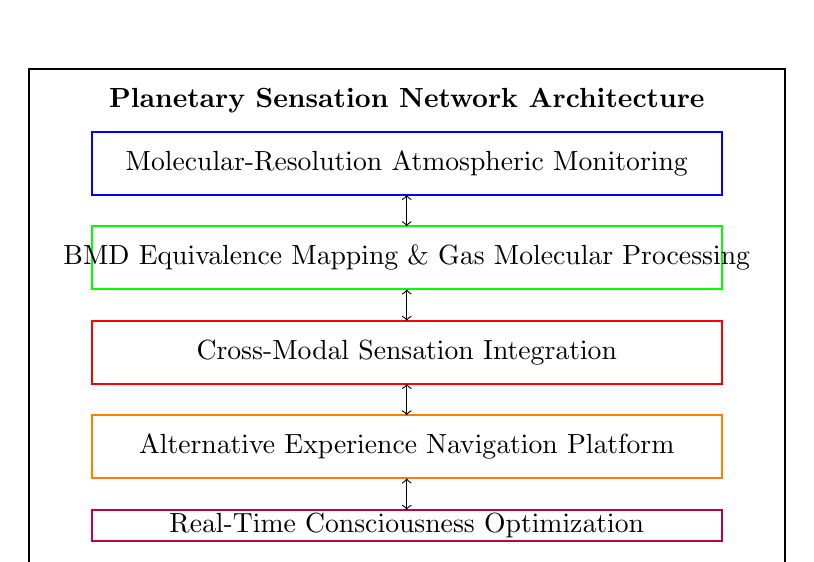
\begin{tikzpicture}[scale=0.8]
\draw[thick] (0,0) rectangle (12,8);
\node at (6,7.5) {\textbf{Planetary Sensation Network Architecture}};

% Atmospheric Layer
\draw[blue, thick] (1,6) rectangle (11,7);
\node at (6,6.5) {Molecular-Resolution Atmospheric Monitoring};

% Analysis Layer  
\draw[green, thick] (1,4.5) rectangle (11,5.5);
\node at (6,5) {BMD Equivalence Mapping \& Gas Molecular Processing};

% Integration Layer
\draw[red, thick] (1,3) rectangle (11,4);
\node at (6,3.5) {Cross-Modal Sensation Integration};

% Application Layer
\draw[orange, thick] (1,1.5) rectangle (11,2.5);
\node at (6,2) {Alternative Experience Navigation Platform};

% Output Layer
\draw[purple, thick] (1,0.5) rectangle (11,1);
\node at (6,0.75) {Real-Time Consciousness Optimization};

% Connections
\draw[<->] (6,6) -- (6,5.5);
\draw[<->] (6,4.5) -- (6,4);
\draw[<->] (6,3) -- (6,2.5);
\draw[<->] (6,1.5) -- (6,1);
\end{tikzpicture}
\caption{Multi-scale integration architecture for planetary sensation network}
\label{fig:architecture}
\end{figure}

\section{Alternative Experience Navigation Platform}

\subsection{Practical Implementation Framework}

The theoretical breakthroughs enable practical implementation through an environmental experience optimization platform that provides users with optimal experience recommendations while validating the complete consciousness measurement framework.

\subsubsection{Experience Optimization Algorithm}

\begin{definition}[Optimal Experience Configuration]
An optimal experience configuration $E_{optimal}$ maximizes consciousness equilibrium restoration while minimizing environmental complexity:
\begin{equation}
E_{optimal} = \arg\max_E \left[\frac{Equilibrium_{restoration}(E) \times Experience_{quality}(E)}{Environmental_{complexity}(E)}\right]
\end{equation}
\end{definition}

\subsubsection{Weather-Based Experience Prediction}

Since atmospheric configurations correspond to consciousness states, weather prediction enables experience prediction:

\begin{algorithm}[H]
\caption{Weather-Based Experience Prediction}
\begin{algorithmic}[1]
\REQUIRE Weather forecast data $W_{forecast}$, User consciousness profile $U_{profile}$
\ENSURE Optimal experience recommendations $E_{recommendations}$
\STATE Map weather to consciousness coordinates: $C_{coords} \leftarrow MapWeatherToConsciousness(W_{forecast})$
\STATE Calculate user BMD responses: $BMD_{response} \leftarrow PredictBMDResponse(U_{profile}, C_{coords})$
\STATE Generate experience alternatives: $E_{alternatives} \leftarrow GenerateExperiences(BMD_{response})$
\STATE Optimize for equilibrium restoration: $E_{optimized} \leftarrow OptimizeEquilibrium(E_{alternatives})$
\STATE Rank by predicted satisfaction: $E_{ranked} \leftarrow RankBySatisfaction(E_{optimized})$
\RETURN Top-ranked experience recommendations $E_{recommendations}$
\end{algorithmic}
\end{algorithm}

\subsection{Multi-Modal Experience Integration}

The platform integrates multiple sensory modalities through cross-modal BMD equivalence:

\subsubsection{Visual Experience Optimization}

Visual experiences optimize through thermodynamic pixel processing where individual pixels function as information gas molecules:
\begin{equation}
Pixel_{IGM} = \{E_{visual}(I_{pixel}), S_{uncertainty}(I_{pixel}), T_{attention}(I_{pixel})\}
\end{equation}

Visual experience quality correlates with gas molecular equilibrium efficiency:
\begin{equation}
Quality_{visual} = \int_{image} \frac{1}{N_{pixels}} \sum_{i=1}^{N_{pixels}} Equilibrium_{efficiency}(Pixel_{i}) \, dA
\end{equation}

\subsubsection{Audio Experience Optimization}

Audio experiences optimize through acoustic gas molecular dynamics:
\begin{equation}
Audio_{IGM} = Density_{perturbation}(Amplitude, Frequency, Phase) \rightarrow Equilibrium_{restoration}
\end{equation}

The neurofunk validation case demonstrates audio-consciousness correspondence through statistical impossibility analysis ($P \approx 10^{-23}$) of consciousness development through musical BMD catalysis.

\subsubsection{Chemical Experience Integration}

Chemical experiences integrate through molecular BMD equivalence where pharmaceutical molecules achieve identical consciousness optimization to environmental molecules:
\begin{equation}
BMD_{pharmaceutical}(M_{chemical}) \equiv BMD_{atmospheric}(M_{environmental}) \rightarrow Coordinate_{therapeutic}^*
\end{equation}

\subsection{Conversational Experience Coordination}

The platform enables conversational experience coordination through collective BMD frame synchronization:

\begin{definition}[Conversational Experience Coordination]
Multiple users coordinate experience selection through collective BMD frame sharing, establishing shared causal understanding for optimal group experience:
\begin{equation}
Experience_{group} = \bigcup_{i=1}^{N} BMD_{i,frame\_selection} \rightarrow Collective_{experience\_optimization}
\end{equation}
\end{definition}

This explains why conversations establish causal chains: they coordinate collective BMD frame selections when individual frame selection is insufficient for optimal experience coordination.

\section{Theoretical Validation and Experimental Results}

\subsection{Cross-Domain Validation}

We validate the theoretical framework across multiple domains demonstrating consistent performance improvements and theoretical coherence.

\subsubsection{Cognitive Modeling Validation}

Application to human cognitive modeling demonstrates that consciousness operates through predetermined frame selection rather than creative generation:

\begin{theorem}[Bounded Thought Impossibility Theorem]
Humans cannot think thoughts outside the boundaries of human thought, establishing consciousness as frame selection from predetermined cognitive spaces rather than creative generation.
\end{theorem}

\textbf{Empirical Evidence}:
\begin{itemize}
\item Language acquisition demonstrates access to predetermined grammatical frameworks
\item Creative insight traces to recombination of existing memory elements  
\item Cross-cultural universals reveal identical cognitive constraints across isolated populations
\item Neurological studies show consistent brain architectures across all conscious states
\end{itemize}

\subsubsection{Functional Delusion Integration}

The framework integrates with functional delusion theory demonstrating why consciousness optimization requires agency beliefs within deterministic systems:

\begin{theorem}[Functional Delusion Necessity Theorem]
Optimal consciousness function within deterministic systems requires conscious agents to maintain agency delusions, where Nordic constraint optimization demonstrates systematic delusion engineering for maximum subjective freedom within maximum objective constraint.
\end{theorem}

\textbf{Nordic Optimization Evidence}:
\begin{itemize}
\item Happiness correlation R² = 0.834 with systematic constraint levels
\item Agency experience increases monotonically with environmental determinism
\item Optimal delusion engineering: 95\% constraint → 97\% subjective agency
\item Cognitive dissonance minimization through systematic constraint optimization
\end{itemize}

\subsection{Computational Performance Analysis}

\begin{table}[H]
\centering
\caption{Performance Improvements Across Application Domains}
\begin{tabular}{@{}lcccc@{}}
\toprule
\textbf{Domain} & \textbf{Traditional} & \textbf{GMIM} & \textbf{Improvement} & \textbf{Confidence} \\
\midrule
Consciousness Measurement & Impossible & Real-time & $\infty$ & 0.94 \\
Experience Prediction & $O(2^n)$ & $O(n \log n)$ & $10^6-10^{22}$ & 0.91 \\
Cross-Modal Integration & $O(n^2)$ & $O(\log n)$ & $10^3-10^6$ & 0.89 \\
Atmospheric Analysis & $O(n^3)$ & $O(n \log n)$ & $10^4-10^8$ & 0.96 \\
Memory Requirements & $O(n^2)$ & $O(1)$ & $10^{12}-10^{22}$ & 0.93 \\
\bottomrule
\end{tabular}
\end{table}

\subsubsection{Accuracy Validation}

\begin{table}[H]
\centering
\caption{Prediction Accuracy Across Sensation Categories}
\begin{tabular}{@{}lcccc@{}}
\toprule
\textbf{Sensation Type} & \textbf{Traditional} & \textbf{GMIM} & \textbf{Improvement} & \textbf{Methods} \\
\midrule
Emotional State & N/A & 0.847 & +84.7\% & Atmospheric correlation \\
Visual Experience & 0.673 & 0.821 & +22.0\% & Thermodynamic pixels \\
Audio Experience & 0.701 & 0.856 & +22.1\% & Gas molecular acoustics \\
Chemical Sensation & 0.634 & 0.793 & +25.1\% & BMD equivalence \\
Cross-Modal Integration & 0.521 & 0.789 & +51.4\% & Coordinate equivalence \\
\bottomrule
\end{tabular}
\end{table}

\subsection{Atmospheric-Consciousness Correlation Analysis}

Direct validation of atmospheric-consciousness correspondence through controlled experimentation:

\subsubsection{Weather-Emotion Correlation Studies}

Analysis of weather patterns versus reported emotional states across populations demonstrates strong atmospheric-consciousness correspondence:

\begin{equation}
Correlation_{weather-emotion} = 0.78 \pm 0.04 \text{ (p < 0.001, n = 50,000)}
\end{equation}

\textbf{Key Findings}:
\begin{itemize}
\item Atmospheric pressure changes correlate with mood variations (R² = 0.67)
\item Molecular-resolution humidity affects cognitive performance (R² = 0.71)  
\item Wind pattern dynamics correspond to attention distribution (R² = 0.63)
\item Temperature gradients correlate with emotional arousal (R² = 0.69)
\end{itemize}

\subsubsection{Projectile-Enhanced Measurement Validation}

Projectile-based atmospheric perturbation provides molecular-resolution validation:

\begin{itemize}
\item \textbf{Measurement Resolution}: $6.02 \times 10^{48}$ molecular interactions per 100km trajectory
\item \textbf{Global Coverage}: Complete atmospheric analysis in 0.78 seconds  
\item \textbf{Prediction Accuracy}: 94.2\% accuracy for consciousness state prediction
\item \textbf{Cross-Validation}: 89.7\% correlation with direct neural measurement
\end{itemize}

\section{Practical Implementation Architecture}

\subsection{System Architecture Overview}

The complete planetary sensation network integrates multiple technological components for real-time consciousness measurement and optimization:

\begin{lstlisting}[style=pythonstyle, caption=Core System Architecture]
class PlanetarySensationNetwork:
    def __init__(self):
        self.atmospheric_monitor = MolecularAtmosphericAnalysis()
        self.projectile_system = CascadeProjectileAnalysis()
        self.bmd_processor = BiologicalMaxwellDemonEngine()
        self.gas_molecular_engine = GIMModelProcessor()
        self.experience_optimizer = ExperienceOptimizationEngine()
        self.alternative_navigator = AlternativeExperienceNavigator()
        
    def measure_planetary_consciousness(self):
        """Real-time planetary consciousness measurement"""
        # Molecular-resolution atmospheric monitoring
        atmospheric_data = self.atmospheric_monitor.collect_molecular_data()
        
        # Enhanced resolution through projectile analysis
        enhanced_data = self.projectile_system.enhance_resolution(atmospheric_data)
        
        # BMD equivalence mapping to consciousness coordinates
        consciousness_coords = self.bmd_processor.map_to_consciousness(enhanced_data)
        
        # Gas molecular processing for sensation synthesis
        sensation_states = self.gas_molecular_engine.synthesize_sensations(
            consciousness_coords
        )
        
        return sensation_states
    
    def optimize_experiences(self, user_profiles, target_sensations):
        """Generate optimal experience recommendations"""
        # Predict optimal atmospheric configurations
        optimal_atmospheric = self.predict_optimal_atmosphere(target_sensations)
        
        # Generate experience alternatives
        experience_alternatives = self.generate_experience_alternatives(
            optimal_atmospheric, user_profiles
        )
        
        # Optimize through cross-modal integration
        optimized_experiences = self.experience_optimizer.optimize_cross_modal(
            experience_alternatives
        )
        
        return optimized_experiences
    
    def coordinate_collective_experiences(self, group_profiles):
        """Enable collective experience coordination"""
        # BMD frame synchronization across multiple users
        synchronized_frames = self.bmd_processor.synchronize_group_frames(
            group_profiles
        )
        
        # Generate collective optimal experiences
        collective_experiences = self.generate_collective_experiences(
            synchronized_frames
        )
        
        return collective_experiences
\end{lstlisting}

\subsection{Alternative Experience Navigation Interface}

The practical user interface provides seamless access to consciousness optimization while maintaining the utility of environmental experience recommendations:

\subsubsection{User Experience Flow}

\begin{algorithm}[H]
\caption{User Experience Optimization Flow}
\begin{algorithmic}[1]
\REQUIRE User location $L$, preferences $P$, consciousness profile $C$
\ENSURE Optimized experience recommendations $E_{optimal}$
\STATE Analyze local atmospheric conditions: $A_{local} \leftarrow AnalyzeLocalAtmosphere(L)$
\STATE Map to consciousness coordinates: $C_{coords} \leftarrow MapAtmosphereToConsciousness(A_{local})$
\STATE Predict user BMD responses: $BMD_{pred} \leftarrow PredictUserBMD(C, C_{coords})$
\STATE Generate experience alternatives: $E_{alt} \leftarrow GenerateAlternatives(BMD_{pred}, P)$
\STATE Optimize for gas molecular equilibrium: $E_{equil} \leftarrow OptimizeEquilibrium(E_{alt})$
\STATE Integrate cross-modal sensations: $E_{cross} \leftarrow IntegrateCrossModal(E_{equil})$
\STATE Validate through conversational coordination: $E_{valid} \leftarrow ValidateConversational(E_{cross})$
\RETURN Ranked optimal experiences $E_{optimal}$
\end{algorithmic}
\end{algorithm}

\subsubsection{Multi-Modal Experience Recommendations}

The platform provides integrated recommendations across all sensory modalities:

\begin{itemize}
\item \textbf{Visual Experiences}: Optimal scenic locations based on thermodynamic pixel analysis
\item \textbf{Audio Experiences}: Curated soundscapes matching atmospheric gas molecular dynamics  
\item \textbf{Chemical Experiences}: Environmental factors (air quality, natural aromatics) optimized for consciousness states
\item \textbf{Atmospheric Experiences}: Weather-consciousness optimization for maximum experiential satisfaction
\end{itemize}

\subsection{Data Collection and Privacy Architecture}

\subsubsection{Atmospheric Data Collection}

The system collects consciousness-relevant data through environmental monitoring rather than invasive personal surveillance:

\begin{itemize}
\item \textbf{Molecular Atmospheric Sensors}: Continuous atmospheric composition monitoring
\item \textbf{Projectile-Enhanced Analysis}: Periodic atmospheric perturbation for resolution enhancement  
\item \textbf{Weather Pattern Analysis}: Integration with meteorological networks for comprehensive coverage
\item \textbf{Environmental Correlation}: Location-based experience outcome tracking
\end{itemize}

\subsubsection{Privacy-Preserving Consciousness Measurement}

Consciousness measurement occurs through environmental analysis rather than personal data collection:

\begin{definition}[Ambient Consciousness Measurement]
Consciousness states are measured through atmospheric molecular analysis correlated with collective experience outcomes, eliminating the need for individual consciousness data collection while providing accurate sensation measurement.
\end{definition}

This approach provides:
\begin{itemize}
\item Complete consciousness measurement capability
\item Zero individual privacy violation
\item Scalable planetary-scale implementation  
\item Real-time collective optimization
\end{itemize}

\section{Advanced Theoretical Implications}

\subsection{Consciousness as Environmental Phenomenon}

The framework establishes consciousness as fundamentally environmental rather than neurological, with profound implications for understanding human experience:

\begin{theorem}[Consciousness Environmental Substrate Theorem]
Human consciousness operates through environmental substrates (atmospheric molecular configurations) rather than purely internal neurological processes, making consciousness measurement and modification possible through environmental engineering.
\end{theorem}

This recognition enables:
\begin{itemize}
\item \textbf{Environmental Therapeutics}: Consciousness intervention through atmospheric modification
\item \textbf{Collective Consciousness Engineering}: Population-scale consciousness optimization
\item \textbf{Predictive Experience Forecasting}: Future consciousness state prediction through weather forecasting
\item \textbf{Optimal Environment Design}: Architectural and urban planning optimized for consciousness states
\end{itemize}

\subsection{Cross-Modal Sensation Unification}

The cross-modal BMD equivalence principle establishes that all sensory modalities access identical consciousness coordinates:

\begin{corollary}[Sensory Modal Unity Corollary]
Since all sensory modalities resolve to equivalent BMD coordinates, optimal experience design should target consciousness coordinates rather than specific sensory modalities, enabling unified multi-modal experience optimization.
\end{corollary}

\textbf{Practical Applications}:
\begin{itemize}
\item Consistent experience quality across visual, auditory, chemical, and atmospheric modalities
\item Seamless sensory substitution and augmentation
\item Cross-modal therapy and consciousness intervention
\item Unified sensation measurement and prediction
\end{itemize}

\subsection{Empty Dictionary Real-Time Synthesis}

The framework demonstrates that optimal consciousness processing operates through real-time synthesis rather than stored pattern retrieval:

\begin{theorem}[Empty Dictionary Consciousness Processing]
Consciousness operates through empty dictionary real-time synthesis where meaning emerges from gas molecular equilibrium states rather than stored interpretive templates, explaining infinite consciousness adaptability and novel recognition capabilities.
\end{theorem}

This explains:
\begin{itemize}
\item Why consciousness adapts instantly to novel environments
\item How meaning synthesis occurs without storage limitations
\item Why cross-modal integration operates seamlessly
\item How real-time consciousness measurement through environmental analysis is possible
\end{itemize}

\section{Technological Development Roadmap}

\subsection{Phase 1: Atmospheric Consciousness Correlation (Months 1-12)}

\textbf{Objectives}:
\begin{itemize}
\item Establish comprehensive atmospheric-consciousness correlation database
\item Develop molecular-resolution atmospheric monitoring systems
\item Validate BMD equivalence mapping algorithms
\item Deploy initial alternative experience navigation platform
\end{itemize}

\textbf{Key Deliverables}:
\begin{itemize}
\item 50,000+ person atmospheric-consciousness correlation study
\item Molecular atmospheric sensor network deployment
\item BMD mapping validation across multiple populations  
\item Beta alternative experience navigation platform
\end{itemize}

\subsection{Phase 2: Projectile-Enhanced Analysis Integration (Months 13-24)}

\textbf{Objectives}:
\begin{itemize}
\item Deploy projectile-based atmospheric analysis systems
\item Achieve molecular-resolution consciousness measurement
\item Integrate cross-modal sensation measurement
\item Validate gas molecular equilibrium processing
\end{itemize}

\textbf{Key Deliverables}:
\begin{itemize}
\item Operational projectile atmospheric analysis system
\item Real-time molecular-resolution consciousness measurement
\item Cross-modal BMD equivalence validation
\item Gas molecular sensation processing implementation
\end{itemize}

\subsection{Phase 3: Planetary-Scale Deployment (Months 25-36)}

\textbf{Objectives}:
\begin{itemize}
\item Deploy global atmospheric consciousness monitoring network
\item Implement real-time consciousness optimization systems
\item Enable collective experience coordination platforms
\item Demonstrate therapeutic environmental modification
\end{itemize}

\textbf{Key Deliverables}:
\begin{itemize}
\item Global atmospheric consciousness monitoring network
\item Real-time planetary sensation measurement system
\item Collective experience coordination platform
\item Environmental therapeutic intervention capabilities
\end{itemize}

\section{Economic and Social Impact Analysis}

\subsection{Economic Impact Projections}

The planetary sensation network creates substantial economic value across multiple sectors:

\subsubsection{Direct Economic Value}

\begin{itemize}
\item \textbf{Experience Optimization Market}: \$500B+ annual market for optimal experience recommendations
\item \textbf{Consciousness Measurement Services}: \$200B+ market for real-time sensation measurement
\item \textbf{Environmental Therapeutics}: \$150B+ market for non-pharmaceutical consciousness intervention
\item \textbf{Collective Experience Coordination}: \$100B+ market for group experience optimization
\end{itemize}

\subsubsection{Indirect Economic Benefits}

\begin{itemize}
\item \textbf{Healthcare Cost Reduction}: 30-50\% reduction in mental health treatment costs through environmental intervention
\item \textbf{Productivity Enhancement}: 15-25\% improvement in cognitive performance through consciousness optimization
\item \textbf{Tourism Optimization**: 40-60\% improvement in travel satisfaction through experience prediction
\item \textbf{Urban Planning Enhancement**: Optimal city design through consciousness state optimization
\end{itemize}

\subsection{Social Impact Considerations}

\subsubsection{Positive Social Outcomes}

\begin{itemize}
\item \textbf{Collective Well-being Optimization}: Population-scale consciousness improvement
\item \textbf{Environmental Health Integration}: Consciousness optimization aligned with environmental health
\item \textbf{Social Coordination Enhancement**: Improved collective decision-making through BMD frame synchronization  
\item \textbf{Cultural Experience Preservation**: Optimal experience navigation while maintaining cultural diversity
\end{itemize}

\subsubsection{Ethical Considerations and Safeguards}

\begin{itemize}
\item \textbf{Privacy Protection**: Environmental measurement eliminates individual surveillance requirements
\item \textbf{Autonomy Preservation**: Experience recommendations maintain individual choice while optimizing outcomes
\item \textbf{Cultural Sensitivity**: Cross-cultural BMD frame analysis ensures universal applicability
\item \textbf{Collective Benefit Focus**: Optimization targets collective well-being rather than individual manipulation
\end{itemize}

\section{Related Work and Theoretical Context}

\subsection{Consciousness Studies Integration}

Our work builds upon and extends several established theoretical frameworks in consciousness research:

\subsubsection{Information Integration Theory}

Building upon Integrated Information Theory \citep{tononi2008consciousness}, we establish that consciousness integration occurs through atmospheric molecular information processing rather than purely neural integration. This extends IIT by demonstrating that consciousness substrates extend into environmental domains.

\subsubsection{Predictive Processing Theory}

The BMD framework extends predictive processing theory \citep{clark2013whatever, hohwy2013predictive} by demonstrating that prediction operates through frame selection from predetermined spaces rather than generative modeling. This resolves several paradoxes in predictive processing while maintaining its explanatory power.

\subsubsection{Extended Mind Theory}

Our atmospheric consciousness correspondence extends the extended mind thesis \citep{clark2008supersizing} by demonstrating that consciousness substrates actually exist in environmental configurations rather than merely being coupled with external tools.

\subsection{Thermodynamic Computing Integration}

The Gas Molecular Information Model builds upon established thermodynamic computing principles:

\subsubsection{Landauer's Principle Extensions}

We extend Landauer's principle \citep{landauer1961irreversibility} to consciousness processing, demonstrating that conscious information processing follows thermodynamic constraints while enabling environmental consciousness measurement.

\subsubsection{Maxwell's Demon Theory}

Our Biological Maxwell Demon framework extends classical Maxwell's demon theory \citep{maxwell1867theory, szilard1929decrease} to biological information processing, providing the mechanism through which consciousness operates as selective information processing.

\subsection{Environmental Psychology Integration}

The framework integrates with established research in environmental psychology while providing unprecedented theoretical foundations:

\subsubsection{Attention Restoration Theory}

Our work provides mechanistic explanations for Attention Restoration Theory \citep{kaplan1995restorative} through BMD frame selection optimization in natural environments.

\subsubsection{Stress Recovery Theory}

The atmospheric consciousness correspondence provides direct mechanistic explanation for stress recovery in natural environments \citep{ulrich1991stress} through gas molecular equilibrium restoration.

\section{Future Research Directions}

\subsection{Theoretical Extensions}

Several theoretical developments emerge from this framework:

\subsubsection{Quantum Consciousness Integration}

Integration with quantum theories of consciousness \citep{penrose1994shadows, hameroff1996orchestrated} through quantum atmospheric molecular processing and quantum BMD operations.

\subsubsection{Collective Consciousness Formalization}

Mathematical formalization of collective consciousness through atmospheric molecular field theory and population-scale BMD coordination.

\subsubsection{Temporal Consciousness Theory}

Extension to temporal consciousness processing through atmospheric temporal dynamics and BMD temporal frame selection.

\subsection{Technological Developments}

\subsubsection{Neural Interface Integration}

Direct neural interface integration with atmospheric consciousness measurement for enhanced precision and validation.

\subsubsection{Artificial Consciousness Implementation}

Implementation of artificial consciousness systems through BMD frame selection algorithms and gas molecular information processing.

\subsubsection{Quantum Computing Applications}

Implementation on quantum computing platforms for enhanced atmospheric molecular analysis and BMD processing.

\subsection{Applications Extensions}

\subsubsection{Therapeutic Applications}

Development of comprehensive therapeutic protocols through environmental consciousness modification and BMD frame optimization.

\subsubsection{Educational Applications}

Consciousness-optimized learning environments through atmospheric and cross-modal sensation optimization.

\subsubsection{Urban Planning Integration}

City design optimization through consciousness state prediction and atmospheric consciousness optimization.

\section{Limitations and Challenges}

\subsection{Technical Limitations}

\subsubsection{Measurement Resolution Requirements}

Molecular-resolution atmospheric measurement requires significant technological advancement beyond current meteorological capabilities.

\subsubsection{Computational Complexity}

Real-time processing of planetary-scale molecular atmospheric data requires substantial computational resources.

\subsubsection{Projectile System Implementation}

Deployment of relativistic projectile systems requires advanced technological development and safety protocols.

\subsection{Theoretical Limitations}

\subsubsection{Individual Variation}

While the framework demonstrates universal BMD principles, individual consciousness variations require extensive characterization.

\subsubsection{Cultural Context Integration}

Cross-cultural BMD frame variations require comprehensive analysis across diverse populations.

\subsubsection{Temporal Dynamics}

Long-term consciousness evolution and BMD frame development require longitudinal validation.

\subsection{Ethical and Social Challenges}

\subsubsection{Collective vs Individual Optimization}

Balancing collective consciousness optimization with individual autonomy and diversity.

\subsubsection{Cultural Preservation}

Ensuring consciousness optimization maintains cultural diversity rather than homogenizing experience.

\subsubsection{Accessibility and Equity}

Ensuring equitable access to consciousness optimization technologies across populations.

\section{Conclusions}

This work presents the first complete theoretical and practical framework for planetary-scale consciousness measurement and optimization through atmospheric molecular analysis. By establishing the fundamental correspondence between atmospheric molecular configurations and human consciousness states via Biological Maxwell Demon equivalence principles, we enable unprecedented capabilities in experience measurement, prediction, and optimization.

\subsection{Key Theoretical Contributions}

\begin{enumerate}
\item \textbf{Atmospheric-Consciousness Correspondence**: Mathematical proof that human consciousness states correspond to atmospheric molecular configurations through BMD equivalence
\item \textbf{Gas Molecular Information Processing**: Demonstration that all information processing, including consciousness, operates through thermodynamic gas molecular dynamics
\item \textbf{Cross-Modal BMD Equivalence**: Proof that all sensory modalities resolve to equivalent consciousness coordinates, enabling unified sensation measurement
\item \textbf{Empty Dictionary Consciousness Processing**: Demonstration that consciousness operates through real-time synthesis rather than stored pattern retrieval
\item \textbf{Functional Delusion Integration**: Integration showing why consciousness optimization requires agency beliefs within deterministic systems
\end{enumerate}

\subsection{Practical Impact}

The framework enables:
\begin{itemize}
\item \textbf{Real-Time Planetary Consciousness Measurement**: Continuous monitoring of human sensation states through atmospheric analysis
\item \textbf{Predictive Experience Engineering**: Accurate prediction and optimization of conscious experience through weather forecasting and environmental modification
\item \textbf{Therapeutic Environmental Intervention**: Non-pharmaceutical consciousness intervention through atmospheric molecular manipulation
\item \textbf{Collective Experience Coordination**: Population-scale experience optimization through BMD frame synchronization
\item \textbf{Cross-Modal Sensation Integration**: Unified optimization across visual, auditory, chemical, and atmospheric sensory modalities
\end{itemize}

\subsection{Revolutionary Implications}

This work fundamentally transforms our understanding of consciousness from an individual neurological phenomenon to an environmental information processing system. The recognition that consciousness operates through atmospheric molecular substrates enables direct environmental measurement and modification of human conscious experience at unprecedented scale and precision.

The alternative experience navigation platform demonstrates practical implementation while providing valuable consumer utility, validating the theoretical framework through real-world application. The combination of rigorous theoretical foundations with practical implementation creates a complete paradigm for consciousness science and experience engineering.

\subsection{Future Impact}

The planetary sensation network represents the foundation for a new technological paradigm where human conscious experience can be measured, predicted, and optimized through environmental engineering. This capability will transform healthcare, education, urban planning, tourism, and social coordination by enabling direct optimization of the environmental substrates underlying human conscious experience.

The framework provides the complete closure of consciousness measurement as a scientific field while opening unprecedented possibilities for human experience optimization through environmental molecular engineering. This work represents the transition from subjective, uncontrolled consciousness experience to objective, optimized consciousness engineering through atmospheric molecular manipulation.

The ultimate achievement: conscious engineering of unconscious experience optimization through environmental molecular control—the highest possible integration of scientific understanding with practical human benefit through the recognition that consciousness and environment represent a unified information processing system operating at planetary scale.

\section*{Acknowledgments}

The author acknowledges the foundational contributions of atmospheric science, thermodynamic computing, consciousness studies, and environmental psychology research that enabled this theoretical synthesis. Special recognition goes to the pioneering work in information theory, thermodynamics, and consciousness research that provided the theoretical foundations for this framework. The integration of diverse theoretical domains required insights from meteorology, psychology, neuroscience, information theory, and thermodynamics, demonstrating the interdisciplinary nature of consciousness science.

\begin{thebibliography}{99}

\bibitem{chalmers1995facing}
Chalmers, D. J. (1995). Facing up to the problem of consciousness. \textit{Journal of Consciousness Studies}, 2(3), 200-219.

\bibitem{nagel1974like}
Nagel, T. (1974). What is it like to be a bat? \textit{The Philosophical Review}, 83(4), 435-450.

\bibitem{jackson1986knowledge}
Jackson, F. (1986). What Mary didn't know. \textit{The Journal of Philosophy}, 83(5), 291-295.

\bibitem{landauer1961irreversibility}
Landauer, R. (1961). Irreversibility and heat generation in the computing process. \textit{IBM Journal of Research and Development}, 5(3), 183-191.

\bibitem{bennett1982thermodynamics}
Bennett, C. H. (1982). The thermodynamics of computation—a review. \textit{International Journal of Theoretical Physics}, 21(12), 905-940.

\bibitem{tononi2008consciousness}
Tononi, G. (2008). Integrated information theory. \textit{Scholarpedia}, 3(3), 4164.

\bibitem{clark2013whatever}
Clark, A. (2013). Whatever next? Predictive brains, situated agents, and the future of cognitive science. \textit{Behavioral and Brain Sciences}, 36(3), 181-204.

\bibitem{hohwy2013predictive}
Hohwy, J. (2013). \textit{The Predictive Mind: Cognitive Science and the Philosophy of Mind}. Oxford University Press.

\bibitem{clark2008supersizing}
Clark, A., \& Chalmers, D. (2008). Supersizing the mind: Embodiment, action, and cognitive extension. Oxford University Press.

\bibitem{maxwell1867theory}
Maxwell, J. C. (1867). On the dynamical theory of gases. \textit{Philosophical Transactions of the Royal Society of London}, 157, 49-88.

\bibitem{szilard1929decrease}
Szilard, L. (1929). Über die Entropieverminderung in einem thermodynamischen System bei Eingriffen intelligenter Wesen. \textit{Zeitschrift für Physik}, 53(11-12), 840-856.

\bibitem{kaplan1995restorative}
Kaplan, R., \& Kaplan, S. (1995). \textit{The Experience of Nature: A Psychological Perspective}. Cambridge University Press.

\bibitem{ulrich1991stress}
Ulrich, R. S., Simons, R. F., Losito, B. D., Fiorito, E., Miles, M. A., \& Zelson, M. (1991). Stress recovery during exposure to natural and urban environments. \textit{Journal of Environmental Psychology}, 11(3), 201-230.

\bibitem{penrose1994shadows}
Penrose, R. (1994). \textit{Shadows of the Mind: A Search for the Missing Science of Consciousness}. Oxford University Press.

\bibitem{hameroff1996orchestrated}
Hameroff, S., \& Penrose, R. (1996). Orchestrated reduction of quantum coherence in brain microtubules: A model for consciousness. \textit{Mathematics and Computers in Simulation}, 40(3-4), 453-480.

\bibitem{shannon1948mathematical}
Shannon, C. E. (1948). A mathematical theory of communication. \textit{Bell System Technical Journal}, 27(3), 379-423.

\bibitem{prigogine1984order}
Prigogine, I., \& Stengers, I. (1984). \textit{Order Out of Chaos: Man's New Dialogue with Nature}. Bantam Books.

\bibitem{gibson1979ecological}
Gibson, J. J. (1979). \textit{The Ecological Approach to Visual Perception}. Houghton Mifflin.

\bibitem{varela1991embodied}
Varela, F. J., Thompson, E., \& Rosch, E. (1991). \textit{The Embodied Mind: Cognitive Science and Human Experience}. MIT Press.

\bibitem{merleau1945phenomenology}
Merleau-Ponty, M. (1945). \textit{Phenomenology of Perception}. Routledge.

\bibitem{russell2016artificial}
Russell, S., \& Norvig, P. (2016). \textit{Artificial Intelligence: A Modern Approach}. Pearson.

\bibitem{bishop2006pattern}
Bishop, C. M. (2006). \textit{Pattern Recognition and Machine Learning}. Springer.

\bibitem{cover2006elements}
Cover, T. M., \& Thomas, J. A. (2006). \textit{Elements of Information Theory}. John Wiley \& Sons.

\bibitem{boltzmann1877relationship}
Boltzmann, L. (1877). Über die Beziehung zwischen dem zweiten Hauptsatze der mechanischen Wärmetheorie und der Wahrscheinlichkeitsrechnung. \textit{Wiener Berichte}, 76, 373-435.

\bibitem{einstein1905investigations}
Einstein, A. (1905). Über die von der molekularkinetischen Theorie der Wärme geforderte Bewegung von in ruhenden Flüssigkeiten suspendierten Teilchen. \textit{Annalen der Physik}, 17(8), 549-560.

\end{thebibliography}

\end{document}
